\documentclass[output=paper,
modfonts,
hidelinks,
newtxmath
]{langscibook}
\bibliography{localbibliography}

% add all extra packages you need to load to this file  
\usepackage{tabularx} 

%%%%%%%%%%%%%%%%%%%%%%%%%%%%%%%%%%%%%%%%%%%%%%%%%%%%
%%%                                              %%%
%%%           Examples                           %%%
%%%                                              %%%
%%%%%%%%%%%%%%%%%%%%%%%%%%%%%%%%%%%%%%%%%%%%%%%%%%%% 
%% to add additional information to the right of examples, uncomment the following line
% \usepackage{jambox}
%% if you want the source line of examples to be in italics, uncomment the following line
% \renewcommand{\exfont}{\itshape}


\usepackage{langsci-gb4e}
\usepackage{langsci-lgr}
\usepackage{langsci-optional}
\usepackage{longtable}
\usepackage{qtree}
\usepackage{slantsc} %needed for slanted smallcaps
\usepackage{multicol}

% \usepackage[polish,czech,english]{babel}
\usepackage{amsmath}
% \usepackage{fontspec}
% \usepackage{unicode-math}
% \usepackage[libertine]{newtxmath}
% \usepackage{libertinus}
\usepackage{stmaryrd}

\usepackage{langsci-cgloss}

% preprint
\usepackage{draftwatermark}
\SetWatermarkText{Preprint}
\SetWatermarkScale{1}
\SetWatermarkColor[rgb]{.94,.94,.94}

%add all your local new commands to this file

\newcommand{\smiley}{:)}

\renewbibmacro*{index:name}[5]{%
  \usebibmacro{index:entry}{#1}
    {\iffieldundef{usera}{}{\thefield{usera}\actualoperator}\mkbibindexname{#2}{#3}{#4}{#5}}}

\newcommand{\un}[1]{$_{\mbox{\scriptsize{#1}}}$} %defines \un as a textmode subscript
\newcommand{\uncnst}[1]{$_{\mbox{\textsf{\tiny{\MakeUppercase{#1}}}}}$}

\DeclareMathSymbol{\Alpha}{\mathalpha}{operators}{"41}
\DeclareMathSymbol{\Mu}{\mathalpha}{operators}{"4D}
\DeclareMathSymbol{\Chi}{\mathalpha}{operators}{"58}

\newcommand{\cnst}[1]{\textsf{\small{\MakeUppercase{#1}}}}


% defining \rightlsquigarrow from MnSymbol

\DeclareFontFamily{U} {MnSymbolA}{}
\DeclareFontShape{U}{MnSymbolA}{m}{n}{
  <-6> MnSymbolA5
  <6-7> MnSymbolA6
  <7-8> MnSymbolA7
  <8-9> MnSymbolA8
  <9-10> MnSymbolA9
  <10-12> MnSymbolA10
  <12-> MnSymbolA12}{}
\DeclareFontShape{U}{MnSymbolA}{b}{n}{
  <-6> MnSymbolA-Bold5
  <6-7> MnSymbolA-Bold6
  <7-8> MnSymbolA-Bold7
  <8-9> MnSymbolA-Bold8
  <9-10> MnSymbolA-Bold9
  <10-12> MnSymbolA-Bold10
  <12-> MnSymbolA-Bold12}{}

\DeclareSymbolFont{MnSyA} {U} {MnSymbolA}{m}{n}

\DeclareMathSymbol{\rightlsquigarrow}{\mathrel}{MnSyA}{160}


% macros for citations:

\newcommand{\citeposst}[1]{\citeauthor{#1}'s (\citeyear{#1})} % produces Chomsky's (1995)
\newcommand{\citeposstpg}[2]{\citeauthor{#1}'s (\citeyear[#2]{#1})} % produces Chomsky's (1995: page)
\newcommand{\citepossalt}[1]{\citeauthor{#1}'s \citeyear{#1}} % produces Chomsky's 1995
\newcommand{\citepossaltpg}[2]{\citeauthor{#1}'s \citeyear[#2]{#1}} % produces Chomsky's 1995: page

% math

% \setmathfont{Libertinus Math}

% keywords

\newcommand{\keywords}[1]{\textbf{Keywords:} {#1}}

% pagenumbering preprint

\pagenumbering{roman}

\papernote{\footnotesize\normalfont
Mojmír Dočekal \& Marcin Wągiel. Event and degree numerals: Evidence from Czech. To appear in: Denisa Lenertová, Roland Meyer, Radek Šimík \& Luka Szucsich (eds.),\textit{ Advances in formal Slavic linguistics 2016}. Berlin: Language Science Press. [preliminary page numbering]
}

\setcounter{chapter}{3}

\title{Event and degree numerals:\newline Evidence from Czech}
 

\author{
 Mojmír Dočekal\affiliation{Masaryk University in Brno}\lastand
 Marcin Wągiel\affiliation{Masaryk University in Brno}
}

% \chapterDOI{} %will be filled in at production
% \epigram{}

\abstract{
In this paper, we bring in novel data concerning the distribution and semantic properties of two classes of adverbs of quantification in Czech, i.e., event numerals such as \textit{dvakrát} `twice/two times' as opposed to degree numerals such as \textit{dvojnásobně} `doubly/twofold'. We explore the contrasts between the expressions in question including the interaction with comparatives and equatives as well as scope asymmetries. We propose that degree numerals target values on a provided scale and are, hence, best analyzed as predicates of degrees whereas event numerals have a more general semantics which primarily allows for quantification over individuated events, but also enables to operate on degrees.

\keywords{numerals, comparative, equative, degrees, scales, events, Czech}
}

\begin{document}
\maketitle
\shorttitlerunninghead{Event and degree numerals}
% \rohead{Event and degree numerals}

\section{Introduction}\label{introduction}

Lexicons of many natural languages distinguish between two types of expressions involving quantification which correspond to English adverbs such as \textit{twice} and \textit{doubly}, see \REF{twice-double-expressions}. Surprisingly, though cardinal numerals have received a lot of attention in the semantic literature on quantification (\citealt{landman2004indefinites}, \citealt{ionin_composition_2006}, \citealt{hofweber2005number}, and \citealt{rothstein2012numericals} among many others), expressions such as those in \REF{twice-double-expressions} remain strikingly understudied both from a descriptive and theoretical perspective (with notable exceptions of \citealt{landman_indefinite_2006}, \citealt{bhatt2007degree}, and \citealt{donazzan_ways_2013}).\footnote{\citet{wagiel-toappear-entities} proposes an analysis of Slavic adjectival multipliers similar to English \textit{double}, however, we are not aware of any semantic treatment of adverbial expressions corresponding to English \textit{doubly}.}

\ea \label{twice-double-expressions} \ea twice/doubly\hfill(English)
\ex deux fois/doublement\hfill(French)
\ex dvaždy/vdvojne\hfill(Russian)
\ex kétszer/kétszeresen\hfill(Hungarian)
\ex hai-lần/gấp-đôi\hfill(Vietnamese)
\z
\z

\noindent The aim of this paper is to present novel data concerning the distribution and semantic properties of such expressions in Czech, exemplified in the text by \REF{twice-double-czech}. In recent years the meaning of different types of Slavic derived numerals has attracted considerable attention (see \citealt{docekal2012atoms,docekal2013numerals} for Czech, \citealt{wagiel2014dwoje,wagiel2015sums} for Polish, and \citealt{khrizman2015cardinal} for Russian), and thus the analysis of the presented data regards a broader enterprise intended to examine numeral quantification from the perspective of morphologically complex languages.

\ea\label{twice-double-czech} \ea \gll dvakrát\label{dvakrat-czech}\\ 
          twice/two.times\\\hfill(Czech)
     \ex \gll dvojnásobně\label{dvojnasobne-czech}\\
          doubly/twofold\\\hfill(Czech)
          \z
\z

\noindent In this paper, we will refer to Czech adverbs of quantification such as \REF{dvakrat-czech} as \textsc{event numerals} (ENs), whereas expressions like \REF{dvojnasobne-czech} will be called \textsc{degree numerals} (DNs). Our goal is primarily empirical, hence we will focus our attention on discussing novel data. More particularly, we will concentrate on constructions in which the degree argument is being manipulated, specifically on the interaction with comparatives and equatives. We claim that ENs are best analyzed as adverbs of quantification whose semantics is general enough to allow for counting distinctive events in terms of iteration as well as operations on degree intervals. On the other hand, DNs are in fact degree predicates which makes their distribution more restricted.

The article is outlined in the following way. In \sectref{distribution}, we will discuss the distribution of Czech ENs and DNs based on the corpus study we have conducted. In \sectref{key-contexts}, we will examine the key environments in which such expressions occur. In \sectref{more-contrasts}, we will focus on categorial and typal differences and we will bring in additional contrasts involving ENs and DNs whereas \sectref{adjectival-and-nominal-degree-numerals} will discuss the properties of adjectival and nominal DNs. \sectref{data-summary} will summarize the data and in \sectref{proposal}, we will propose a predicative semantics for DNs as well as suggest an analysis of ENs. \sectref{conclusion} concludes the paper.

\section{Distribution}\label{distribution}

At first blush, Czech numerals such as \textit{dvakrát} `twice/two times' and \textit{dvojnásobně} `doubly/twofold' appear to be synonymous in some contexts.

\ea \ea \gll Petrovi se to vyplatilo \textbf{dvakrát} / \textbf{dvojnásobně}.\\
for.Petr \textsc{refl} this paid.off twice {} doubly\\
\glt `For Petr it paid off twice.'
\ex \gll Ceny tady jsou \textbf{dvakrát} / \textbf{dvojnásobně} vyšší než tam.\\
prices here are twice {} doubly higher than there\\
\glt `The prices here are two times higher than there.'
\z
\z

\noindent However, a more careful investigation reveals that there are multiple environments in which they are not. In order to determine the distribution of ENs and DNs and to define the properties of the contexts in which they occur, we conducted a corpus study based on the Czech National Corpus (CNC).\footnote{The CNC is a representative corpus of contemporary Czech. We have selected the SYN2015 subcorpus \citep{kren-etal2015}, which is the largest reference corpus of contemporary written Czech consisting of more than 100 million tokens. We searched for the lemmas \textit{dvakrát} and \textit{dvojnásobně}.} The selected corpus samples contained 100 random occurrences of the EN \textit{dvakrát} and the DN \textit{dvojnásobně}, which were reduced to 98 and 99 occurrences, respectively, after filtering. Figures \ref{fig:distr_dvakrat} and \ref{fig:distr_dvojnasobne} present the preferred environments in which the numerals in question appear in the samples.

\begin{figure}[t]
\captionof{figure}{Distribution of \textit{dvakrát}}\label{fig:distr_dvakrat}

\footnotesize
\barplot{}{}{VP,COMP/EQ,AdvP,AP,PP,Clause}%
{
(VP,61)
(COMP/EQ,12)
(AdvP,8)
(AP,7)
(PP,7)
(Clause,3)
}
\end{figure}

\normalsize
\begin{figure}
\caption{Distribution of \textit{dvojnásobně}}
\footnotesize
\label{fig:distr_dvojnasobne}
\barplot{}{}{COMP,VP,AP,Secondary predication,AdvP}%
{
(COMP,31)
(VP,30)
(AP,22)
(Secondary predication,14)
(AdvP,2)
}
\end{figure}
\normalsize

% \vspace{7mm}
% \begin{minipage}[b]{.48\textwidth}
% \centering
% 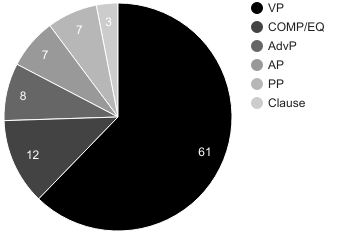
\includegraphics[width=\linewidth]{graph_1.png}
% \captionof{figure}{Distribution of \textit{dvakrát}}
% \label{fig:distr_dvakrat}
% \end{minipage}
% \begin{minipage}[b]{.48\textwidth}
% \centering
% 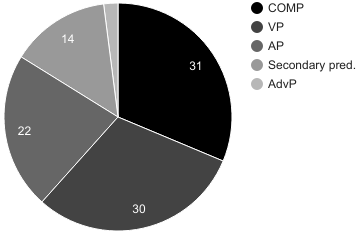
\includegraphics[width=\linewidth]{graph_2.png}
% \captionof{figure}{Distribution of \textit{dvojnásobně}}
% \label{fig:distr_dvojnasobne}
% \end{minipage}

\noindent The results show a significant difference in the distribution of ENs and DNs that, in our opinion, unveils the real nature of these expressions. Whereas in 77\% of occurrences, \textit{dvakrát} targets event-denoting VPs as well as temporal AdvPs and PPs,\footnote{Following \cite{doetjes_adverbs_2007}, we assume that adverbials such as \textit{dvakrát denně} `twice a day' and \textit{dvakrát za týden} `twice a week' are similar to frequency expressions in the sense that their interpretation is dependent on the time interval they introduce.} \textit{dvojnásobně} tends to modify comparatives, APs, and secondary predicates as well as degree-related VPs.\footnote{Out of 30 VPs modified by \textit{dvojnásobně} 9 were headed by deadjectival verbs, e.g., \textit{zvětšit} `enlarge' and \textit{zvýšit} `raise', whereas 11 involved predicates inherently associated with scales including verbs operating on degrees such as \textit{zvednout} and \textit{vzrůst} `increase'. The remaining 10 examples involved predicates such as \textit{platit} `pay', \textit{trestat} `punish', and \textit{jásat} `rejoice' which arguably at least to some extent also pertain to the notion of gradability.} In total, it targets scales in 90\% of the studied cases. The observed contrast suggests that \textit{dvakrát} naturally favors event-denoting environments (though it can appear in comparatives and equatives) whereas \textit{dvoj\-násobně} exhibits a very strong tendency to select for degree expressions.

In the following sections, we will examine two contexts we assume to be crucial for understanding the character of the EN/DN alternation as well as further contrasts and differences between those expressions.

\section{Key contexts}\label{key-contexts}

\subsection{Degrees and differentials}\label{degrees-and-differentials}

The first environment to be discussed is constituted by degree constructions involving comparison. Both ENs and DNs can appear in comparatives as differentials, as attested by the examples from the CNC corpus in \REF{comparatives-cnc}.

\ea\label{comparatives-cnc} \ea \gll {\ldots} je dnes až \textbf{dvojnásobně} větší nebezpečí ničivých
povodní než před 20 lety.\\
{} is today even doubly bigger danger destructive floods than before 20
years\\\hfill(CNC)
\glt `{\dots} today, the danger of destructive floods is two times bigger than 20
years ago.'
\ex \gll {\dots} a tak se dokážou \textbf{dvakrát} rychleji ohřát nebo zchladit než
běžné žehličky.\\
{} and thus \textsc{refl} manage twice faster heat or cool.down than ordinary
irons\\\hfill(CNC)
\glt `{\dots} and thus they can heat or cool down two times faster than ordinary
irons.'
\z
\z

\noindent Furthermore, both ENs and DNs are unacceptable in superlatives.\footnote{ENs may appear as superlative modifiers, e.g., in the past tense. However, a sentence such as \textit{Petr byl \textbf{dvakrát} nejvyšší} `Petr was the tallest twice' has only an event reading which states that there were two occasions on which Petr was the tallest one among the compared individuals. Therefore, it seems that in such cases the EN modifies the whole phrase, i.e., the copula and the superlative, rather than the superlative alone.}

\ea *\gll Petr je \textbf{dvakrát} / \textbf{dvojnásobně} nejvyšší.\\
Petr is twice {} doubly tallest\\
\z

\noindent Nevertheless, an interesting contrast arises when we consider equatives. Though Czech ENs are perfectly fine in such an environment, see \REF{dvakrat-comp-eq}, DNs are significantly less acceptable in equatives than in comparatives, as witnessed by the oddity of \REF{dvojnasobne-eq}.\footnote{A similar contrast between \textit{twice} and \textit{two times} in English has been observed in \cite{gobeski2011twice}.} In addition, there are no attested occurrences of equatives with DNs in CNC.

\ea\label{dvakrat-comp-eq} \ea[]{\gll Petr je \textbf{dvakrát} vyšší než Marie.\\
Petr is twice taller than Marie\\
\glt `Petr is two times taller than Marie.'}
\ex[]{\gll Petr je \textbf{dvakrát} tak vysoký jako Marie.\label{dvakrat-eq}\\
Petr is twice so tall how Marie\\
\glt `Petr is twice as tall as Marie.'}
\z \z

\ea \ea[]{\gll Petr je \textbf{dvojnásobně} vyšší než Marie.\label{dvojnasobne-comp}\\
Petr is doubly taller than Marie\\
\glt `Petr is two times taller than Marie.'}
\ex[*]{\gll  Petr je \textbf{dvojnásobně} tak vysoký jako Marie.\label{dvojnasobne-eq}\\
Petr is doubly so tall how Marie\\ }
\z \z

\noindent This property of DNs corresponds to the behavior of standard differentials, which, as indicated in \REF{diff}, although frequently attested in comparatives, are not possible in equatives.\footnote{As an anonymous reviewer points out it seems that \REF{diff-eq} is out because equatives need to apply the AP internally, before the degree variable \textit{d} is bound, for instance by the \cnst{pos} operator (e.g., \citealt{kennedy_mcnally2005scale}).}

\ea \label{diff} \ea[]{\gll Petr je \textbf{o} \textbf{10} \textbf{cm} vyšší než Marie.\\
Petr is by 10 cm taller than Marie\\
\glt `Petr is 10 cm taller than Marie.'\label{diff-comp}}
\ex[*]{\gll Petr je \textbf{o} \textbf{10} \textbf{cm} tak vysoký jako Marie.\\
Petr is by 10 cm so tall how Marie\label{diff-eq}\\ }
\z \z

\noindent These data seem to suggest that though both ENs and DNs can operate on scales, they differ in that they employ distinct strategies to modify the degree they target. On the basis of the presented evidence, we assume it is plausible to hypothesize that DNs share core semantic properties with differentials. On the other hand, the compatibility of ENs with equatives seems to imply that they are expressions of a very distinct type.

\subsection{Count events}\label{count-events}

The second key environment to be discussed here involves VPs referring to individuated count events. Multiple examples attested in the CNC corroborate the well-known fact that ENs can combine with VPs in order to quantify over eventualities. Interestingly, as witnessed by the ungrammaticality of \REF{dvojnasobne-count-events}, DNs cannot be used to count events.

\ea \ea[]{\gll \textbf{Dvakrát} se přesvědčím, že jsou dvířka zavřená.\\
twice \textsc{refl} I.will.ensure that are door closed\\\hfill(CNC)
\glt `I will make sure twice that the door is closed.'}
\ex[*]{\gll \textbf{Dvojnásobně} se přesvědčím, že jsou dvířka zavřená.\label{dvojnasobne-count-events}\\
doubly \textsc{refl} I.will.ensure that are door closed\\ }
\z \z

\noindent Not surprisingly, neither ENs nor DNs modify VPs denoting homogeneous eventualities such as static states, as demonstrated in \REF{states}. As expected, no such examples were found in the CNC samples.

\ea[*]{\gll Petr \textbf{dvakrát} / \textbf{dvojnásobně} zná Marii.\label{states}\\
Petr twice {} doubly knows Marie\\ }
\z

\noindent Another observation concerns VPs referring to values on scales. While both ENs and DNs can modify verbs such as \textit{vzrůst} `increase', there is an asymmetry with respect to possible readings of sentences containing such phrases. Let us consider the contrast between \REF{dvojnasobne-increase} from the CNC and the corresponding example in \REF{dvakrat-increase}. As indicated in the translation, \REF{dvakrat-increase} is ambiguous between the quantified-degree and the quantified-event interpretation, i.e., it is either true of a scenario where the demand increased by two times irrespective of the number of times it increased, or of a situation where there were two events of increasing the demand, irrespective of the value by which the demand was increased. Crucially, \REF{dvojnasobne-increase} lacks the quantified-event interpretation and can only be true of a scenario in which the degree of increase was multiplied by two.

\ea \ea \gll Poptávka po dotacích vzrostla \textbf{dvakrát}.\label{dvakrat-increase}\\
demand after subsidies increased twice\\
\glt `The demand for subsidies increased twice / by two times.'
\ex \gll Poptávka po dotacích vzrostla \textbf{dvojnásobně}.\label{dvojnasobne-increase}\\
demand after subsidies increased doubly\\\hfill(CNC)
\glt `The demand for subsidies increased doubly.'
\z \z

\noindent The discussed observations further support the semantic nature of the EN/DN alternation. At this point, it seems innocuous to state that the distinction relies on the strategy the expressions in question make use of in terms of quantification. Whereas DNs are unable to count events and are restricted to operations on degrees, ENs seem to employ a more general semantics which allows for quantification over both events and degrees. Further differences will be examined in the next section.

\section{More contrasts}\label{more-contrasts}

\subsection{Categorial differences}\label{categorial-differences}

Another difference between Czech ENs and DNs concerns their derivational potential. Both classes involve morphologically complex expressions derived from a numeral root, e.g., \textit{dv-} (corresponding to English \textit{tw-}), by different suffixes, i.e., \textit{-krát} and \textit{-násobn-}.\footnote{In fact, \textit{-násobn-} can be further decomposed at least to \textit{-násob-}, as attested in \textit{násobit} `multiply', and \textit{-n-}. For the sake of simplicity, we will ignore the morphological complexity here.} However, the contrast between \REF{dvakrat-morphology} and \REF{dvojnasobne-morphology} indicates an apparent categorial asymmetry. Unlike DNs, which employ distinct morphology to display a broad range of syntactic categories including adverbial, adjectival, and nominal forms (all derived from the same stem), ENs are defective in the sense that they have only adverbial forms and cannot appear in syntactic contexts which are sensitive for adjectives and nominals.\footnote{It should be noted that the inability of ENs to take adjectival and nominal morphology seems to be a Czech idiosyncrasy since, for instance, Polish allows for forms such as \textit{dwukrotny} `twice.A' and \textit{dwukrotność} `twice.N'. Similar, there is adjectival \textit{dvukratnyj} in Russian and \textit{dvakratni} in Slovenian. However, a detailed cross-linguistic comparison of ENs and DNs is beyond the scope of this paper and constitutes a challenge for further research.}


\begin{multicols}{2}
% \begin{minipage}[t]{0.5\textwidth}
\ea \textit{dvakrát}\label{dvakrat-morphology}
\ea[]{\gll pršelo dvakrát\\
rained twice\\\hfill\textbf{Adv}
\glt `it rained twice'}
\ex[*]{\gll dvakrát(ní) objem\\
twice.A capacity\\\hfill\textbf{A}
\glt {\color{white}I}}
\ex[*]{\gll dvakrát(ek) rychlosti\\
twice.N speed\\\hfill\textbf{N}
\glt {\color{white}I}}

\z
\z
\columnbreak
% \end{minipage}
%
% \begin{minipage}[t]{0.5\textwidth}
\ea \textit{dvojnásob-}\label{dvojnasobne-morphology} 
\ea \gll dvojnásobně dlouhý\\
doubly long\\\hfill\textbf{Adv}
\glt `two times longer'
\ex \gll dvojnásobný objem\\
double capacity\\\hfill\textbf{A}
\glt `double the capacity'
\ex \gll dvojnásobek ceny\\
double.N price\\\hfill\textbf{N}
\glt `double the price'
\z \z

\end{multicols}
% \end{minipage}
\vspace{3mm}

\noindent Although the categorial asymmetry provided in \REF{dvakrat-morphology} and \REF{dvojnasobne-morphology} may suggest that ENs and DNs are exponents of distinct semantic objects, as such it is, of course, insufficient to draw a typal distinction between the two. In the next section, we will investigate such a possibility in more detail.

\subsection{Typal compatibility}\label{typal-compatibility}

A further observation concerns the fact that ENs and DNs in Czech can be stacked, as witnessed by the grammaticality of examples such as \REF{stacked-numerals}. This suggests that Czech expressions of those kinds are compatible in terms of their semantic types. Moreover, the reversed order of numerals, as provided in \REF{stacked-numerals-*}, is not possible, which further suggests different input requirements.

\ea \ea[]{\gll Petrovi se to \textbf{třikrát} \textbf{dvojnásobně} vyplatilo.\label{stacked-numerals}\\
for.Petr \textsc{refl} this thrice doubly paid.off\\
\glt `For Petr it paid off doubly three times.'}
\ex[*]{\gll Petrovi se to \textbf{dvojnásobně} \textbf{třikrát} vyplatilo.\label{stacked-numerals-*}\\
for.Petr \textsc{refl} this doubly thrice paid.off\\ }
\z \z

\noindent Furthermore, there is solid evidence that unlike ENs, DNs are anchored to a particular event. Let us consider possible interpretations of a sentence such as \REF{stacked-numerals-int} in which the conjoined NP in subject position denotes a plurality of entities whereas the modified VP refers to a plurality of events. As indicated in \REF{stacked-numerals-int-a} and \REF{stacked-numerals-int-b}, the sentence can either have a distributive reading where the events of paying off doubly are distributed equally onto each of the individuals, i.e., Petr and Honza, or a collective reading in which it payed off doubly three times for Petr and Honza as a group. Moreover, a cumulative interpretation as in \REF{stacked-numerals-int-c} is also possible. In such a scenario there was a total of three events of paying off doubly and Petr and Honza share the total gain disproportionately. Nevertheless, \REF{stacked-numerals-int} cannot have a meaning such as the one in \REF{stacked-numerals-int-d} or in \REF{stacked-numerals-int-e}. It is impossible to understand the sentence in such a way that the total gain corresponds to six units, similar to \REF{stacked-numerals-int-b} or \REF{stacked-numerals-int-c}, but the total number of events is less or greater than three. Such cumulations are simply unaccessible which implies that DNs cannot outscope the event quantifier and are forced to operate on degrees within a particular event.

\ea\label{stacked-numerals-int} 
\gll Petrovi a Honzovi se to \textbf{třikrát} \textbf{dvojnásobně} vyplatilo.\\
for.Petr and for.Honza \textsc{refl} this thrice doubly paid.off\\
\glt `For Petr and Honza it paid off doubly three times.'
\ea[]{for Petr: 3 $\times$ (it-paid-off $\times$ 2) $+$ for Honza: 3 $\times$ (it-paid-off $\times$ 2)\label{stacked-numerals-int-a}}
\ex[]{for Petr$+$Honza: 3 $\times$ (it-paid-off $\times$ 2)\label{stacked-numerals-int-b}}
\ex[]{for Petr: 2 $\times$ (it-paid-off $\times$ 2) $+$ for Honza: 1 $\times$ (it-paid-off $\times$ 2)\label{stacked-numerals-int-c}}
\ex[*]{for Petr$+$Honza: 2 $\times$ (it-paid-off $\times$ 3)\label{stacked-numerals-int-d}}
\ex[*]{for Petr: 4 $\times$ (it-paid-off $\times$ 1) $+$
for Honza: 1 $\times$ (it-paid-off $\times$ 2)\label{stacked-numerals-int-e}}
\z \z

\noindent The data clearly demonstrate that adverbial ENs and DNs differ with respect to their semantic type and scopal properties. The following sections will explore some additional semantic phenomena related to adjectival and nominal forms of DNs.

\section{Adjectival and nominal degree numerals}\label{adjectival-and-nominal-degree-numerals}

\subsection{Quantification over amounts and values}\label{quantification-over-amounts}

Let us now consider Czech adjectival DNs such as \textit{dvojnásobný} `double/two-time'. The CNC data confirm our intuition that such expressions often modify amount nominals and nouns implicitly associated with scales like those in \REF{dvojnasobny-amount-scales}.\footnote{In the CNC, among the 15 most frequent collocation candidates for the lemma \textit{dvojnásobný} (1,567 occurrences in SYN2015) one can find the followings nouns: \textit{počet} `number', \textit{množství} `amount', \textit{cena} `price', and \textit{rychlost} `speed'.} In those contexts, the DN appears to multiply a contextually provided value on a particular scale. As a result, the predicates in \REF{dvojnasobny-amount-scales} are true of a twice as high volume and a twice as high salary, respectively.

\ea\label{dvojnasobny-amount-scales} \ea \gll dvojnásobný objem\label{dvojnasobny-objem}\\
double volume\\
\glt `double the volume'
\ex \gll dvojnásobný plat\\
double salary\\
\glt `double the salary'
\z  \z

\noindent Interestingly, adjectival DNs are not compatible with container nouns, as the contrast between \REF{dvojnasobny-amount} and \REF{dvojnasobny-container} shows. This property differentiates them from basic cardinal numerals, since in order to quantify over amounts determined by container nominals Czech requires cardinals to do the job, see \REF{dvakrat-container}. Czech cardinals, however, are unable to combine with amount nouns to count quantities, as witnessed by the ungrammaticality of \REF{dvakrat-amount}.

\ea \ea[]{\gll dvojnásobné množství čaje\label{dvojnasobny-amount}\\
double amount tea\\
\glt `double the amount of tea'}
\ex[*]{\gll dvojnásobný hrnek čaje\label{dvojnasobny-container}\\
double cup tea\\ }
\ex[]{\gll dva hrnky čaje\label{dvakrat-container}\\
two cups tea\\
\glt `two cups of tea'}
\ex[*]{\gll dvě množství čaje\label{dvakrat-amount}\\
two amount tea\\ }
\z \z

\noindent The data discussed above show that DNs and cardinals are in complementary distribution with respect to container and amount nouns. This fact suggests that the two types of expressions in question make use of distinct quantificational strategies and should be analyzed differently.

\subsection{Events and social roles}\label{events-and-social-roles}

Amount nouns do not exhaust the combinatorial potential of adjectival DNs since they can also modify two other classes of expressions, specifically nominals referring to events, as exemplified in \REF{dvojnasobna-vrazda}, as well as nominals denoting social functions such as, e.g., family roles and public capacities, see \REF{dvojnasobny-mistr}.\footnote{The CNC collocation candidates list includes, among others, the following examples for the first class: \textit{vražda} `murder', \textit{přesilovka} `power play', and \textit{radost} `joy', as well as \textit{vítěz} `winner', \textit{matka} `mother', and \textit{účastník} `participant' for the latter.} Nevertheless, the interpretation of such phrases differs from the meaning of, e.g., \REF{dvojnasobny-amount-scales}, in which the DN seems to merely multiply the value indicated by the implicit degree argument of the amount nominal. For instance, \REF{dvojnasobna-vrazda} refers to a set of murdering events involving two victims in each such an event, i.e., the DN seems to access an internal argument of the deverbal nominal. On the other hand, similar to what was observed in \citet{wagiel2015multiplicative} examples such as \REF{dvojnasobny-mistr} denote a set of individuals that have gained a particular property two times -- in this case, the property of becoming a champion.\footnote{Notice that such behavior seems to be a Czech idiosyncrasy since many other languages make use of a different adjective to express such a meaning, e.g., see the English translation in \REF{dvojnasobny-mistr}.}

\ea \label{dvojnasobny} \ea \gll\label{dvojnasobna-vrazda}dvojnásobná vražda\\
double murder\\
\glt `double murder'
\ex \gll dvojnásobný mistr\label{dvojnasobny-mistr}\\
double champion\\
\glt `two-time champion'
\z \z

\noindent Further evidence that amount NPs and nominals implicitly associated with scales substantially differ from nominals denoting events or social roles modified by adjectival DNs comes from the distribution of nominal DNs such as \textit{dvojnásobek} `double.N'. As demonstrated in \REF{dvojnásobek}, such nominalizations cannot take expressions referring to events or social roles as their complements though they frequently combine with amount nominals.\footnote{For instance, the CNC lists the following among the 15 most frequent collocation candidates for the lemma \textit{dvojnásobek} (845 hits in SYN2015): \textit{cena} `price', \textit{částka} `sum of money', \textit{počet} `number', and \textit{velikost} `quantity'.}

\ea\label{dvojnásobek} \ea[]{\gll dvojnásobek rychlosti\\
double.N speed\\
\glt `double the speed'}
\ex[*]{\gll dvojnásobek vraždy / mistra\\
double.N murder {} champion\\ }
\z \z

\noindent Moreover, the asymmetry is further supported by the contrast in \REF{dvojnasobny-asymmetry}. In such examples, \textit{je} `is' is not used as a copula of predication, but rather it seems to establish the identity relation between the denotation of its complement and that of the subject NP.\footnote{Note that \REF{dvojnasobna-rychlost} is ungrammatical with the instrumental \textit{rychlostí} `speed.\textsc{ins}', which is commonly associated with predication.} In \REF{dvojnasobna-rychlost}, the definiendum, i.e., the modified degree noun, is associated with the definiens comprising the comparative construction. On the other hand, \REF{dvojnasobny-mistr-je} and \REF{dvojnasobna-sebevrazda} are odd since neither \textit{mistr} `champion', nor \textit{sebevražda} `suicide' provides a degree argument to be accessed by the DN, and thus the subject NPs are not equivalent to the corresponding comparatives. In other words, since the subjects and the nominals within the matrix predicates in \REF{dvojnasobny-mistr-je} and \REF{dvojnasobna-sebevrazda} refer to different entities, establishing the identity relation is impossible.\footnote{This property seems to resemble some sort of a monotonicity constraint, as discussed in \cite{schwarzschild2002grammar}. However, the exact nature of this phenomenon requires further investigation.}

\ea\label{dvojnasobny-asymmetry} \ea[]{\gll \textbf{Dvojnásobná} rychlost je \textbf{dvakrát} větší rychlost.\label{dvojnasobna-rychlost}\\
double speed is twice bigger speed\\
\glt `Double the speed means two times higher speed.'}
\ex[\#]{\gll \textbf{Dvojnásobný} mistr je \textbf{dvakrát} větší mistr.\label{dvojnasobny-mistr-je}\\
double champion is twice bigger champion\\ }
\ex[\#]{\textbf{Dvojnásobná} sebevražda je \textbf{dvakrát} větší sebevražda.\label{dvojnasobna-sebevrazda}\\
double suicide is twice bigger suicide\\ }
\z \z

\noindent The contrasts described above indicate that adjectival and nominal DNs display heterogeneous behavior in interaction with NPs implicitly associated with scales on the one hand and with event and social role nominals on the other. Possibly, the relationship between the two types of phrases is much less straightforward than it might initially seem. In this paper, however, we are primarily concerned with examples such as \REF{dvojnasobny-objem} and we assume that use of adjectival DNs to be the basic one.

\subsection{Predicate position}\label{predicate-position}

Finally, the last observation concerns the attributive and predicative use of adjectival DNs. In all the examples provided in the previous sections, \textit{dvojnásobný} appears as a nominal modifier which seems to be the most natural syntactic context for such an expression. Nevertheless, it is not unusual to find \textit{dvojnásobný} in predicate position as well, as attested in an CNC sentence in \REF{dvojnasobny-predicate}. Here, the DN serves as the main predicate of a sentence and assigns a property to a subject denoting an amount, i.e., \textit{hodnota} `value'. In particular, it is predicated of the value of saved property it is twice as high relative to the value corresponding to the damages, i.e., it amounts to {100 000 CZK}.

\ea \gll {\dots} škoda dosahuje asi 50 tisíc korun. Hodnota uchráněného majetku je \textbf{dvojnásobná}.\label{dvojnasobny-predicate}\\
{} damage reaches approximately 50 thousand crowns value saved property is double\\\hfill(CNC)
\glt `{\dots} the damages reach approximately 50 000 CZK. The value of saved property is twice as high.'
\z

\noindent Sentences such as \REF{dvojnasobny-predicate} are far less frequent in the CNC than examples with adjectival DNs in attributive position. However, we regard their existence as an important piece of evidence, supporting the predicative nature of DNs.

\section{Data summary}\label{data-summary}

Before we move on to the analysis of the EN/DN distinction, let us briefly recapitulate the empirical findings. \tabref{table:properties} summarizes the observed contrasts.\footnote{The most frequent environments based on the CNC corpus study are in bold.} In brief, ENs are able to target both events and degrees. They have only adverbial forms and tend to appear in eventive environments though they can also modify degree constructions including comparatives and equatives. On the other hand, DNs cannot scope over events and they heavily favor scalar contexts excluding equatives. Not only can they take adverbial and nominal, but also adjectival morphology and as such they can quantify over amounts, arguments of events, as well as time intervals associated with social roles specified by nominals they modify. In the next sections, we attempt to account for at least some of the puzzling differences between the two classes of expressions in question. We will propose an analysis of adverbial DNs and suggest possible directions of development to account for the meaning of ENs as well as adjectival DNs.

\begin{table}[t]
\caption{Properties of event and degree numerals}\label{table:properties}
\begin{tabularx}{\textwidth}{@{}lll@{}}
\lsptoprule
Property & Event numerals & Degree numerals\tabularnewline
\midrule
Morphology & Adv & Adv/A/N\tabularnewline
Degree & yes & \textbf{yes}\tabularnewline
Differential in comparatives & yes & \textbf{yes}\tabularnewline
Differential in superlatives & no & no\tabularnewline
Differential in equatives & yes & no\tabularnewline
Modify count events & \textbf{yes} & no\tabularnewline
Modify degree events & yes & yes\tabularnewline
Events (N) & no & yes\tabularnewline
Roles (N) & no & yes\tabularnewline
\lspbottomrule
\end{tabularx}
\end{table}



\section{Proposal}\label{proposal}

\subsection{Degree numerals}\label{degree-numerals}

On the basis of the distributional evidence, we argue that the comparative examples introduced in \sectref{degrees-and-differentials} reveal the true nature of DNs. Let us now consider more closely the example in \REF{dvojnasobne-comp}, repeated here as \REF{comp-ex}. The truth conditions of the sentence are specified informally in \REF{comp-ex-int-a} and \REF{comp-ex-int-b} gives an exemplary situation in which the sentence would be true.

\ea\label{comp-ex} \gll Petr je \textbf{dvojnásobně} vyšší než Marie.\\
Petr is doubly higher than Marie\\
\glt `Petr is two times taller than Marie.'
\ea True in all situations where the height of Petr is qual to the height of Marie multiplied by 2\label{comp-ex-int-a} 
%\b. $\mu_{\textit{\textsc{height}}}(Petr) = 180 \wedge \mu_{\textit{\textsc{height}}}(Marie) = 90$
\ex $\mu$\uncnst{height}(\textsc{Petr}$) = 180 \wedge \mu$\uncnst{height}(\textsc{Marie}$) = 90$\label{comp-ex-int-b}
\z \z

\noindent Building on the observations discussed in \sectref{degrees-and-differentials}, we acknowledge that DNs seem to behave similarly to differentials in that they define the difference between compared values on a scale provided by the comparative. Nonetheless, we argue that the underlying mechanism which yields such a result is distinct. DNs differ from typical differentials in that they do not determine the gap in terms of some absolute value, e.g., 10 cm as in \REF{diff-comp}. Instead, they provide information about the degree corresponding to a correlate in terms of the value related to a standard of comparison. For instance, in \REF{comp-ex} the DN specifies the height of the correlate, i.e., Petr, in terms of the multiplied height of the standard of comparison, i.e., Marie.

We are now ready for the first approximation. Based on the observation discussed in \sectref{predicate-position}, namely that \textit{dvojnásobný} can occur in predicate position, see \REF{dvojnasobny-predicate}, we propose that the primary interpretation DNs have is the predicative one. Furthermore, based on the morphological evidence examined in \sectref{categorial-differences}, we assume that Czech DNs are compositional. We posit that numeral roots simply refer to numbers modeled as abstract entities and as such are expressions of type $n$. On the other hand, the suffix \textit{-násobn-} introduces an operation involving multiplication of a degree by a number denoted by the root. Therefore, we model DNs as degree predicates, i.e., expressions denoting a characteristic function of degrees (type $\langle d,t\rangle$). We posit that such a function yields the truth value True iff a selected degree $d$ is two times higher than some contextually determined value $g$. The semantics for \textit{dvojnásobný} is proposed in \REF{degree-num-semantics-dvojnasobne} whereas \REF{degree-num-semantics-abstract} gives the abstracted meaning of DNs in general.

\ea\label{degree-num-semantics}
\ea $\llbracket$dvojnásobně$\rrbracket = \lambda d[d = 2 \times g]$\hfill{type $\langle d,t\rangle$}\label{degree-num-semantics-dvojnasobne}
\ex $\llbracket$Degree Numeral$\rrbracket = \lambda n\lambda d[d = n \times g]$\hfill{type $\langle n,\langle d,t\rangle\rangle$}\label{degree-num-semantics-abstract}
\z \z

\noindent Let us now consider how \REF{degree-num-semantics-dvojnasobne} accounts for the meaning of \REF{dvojnasobny-predicate}. The denotation of the subject NP (an expression of type $d$), i.e., the value of saved property, has the property of being equal to the value corresponding to the damages multiplied by two. The logical type of the DN is $\langle d,t\rangle$, hence the composition of \REF{dvojnasobny-predicate} proceeds via the standard rule of Function Application. The predicate of degrees is applied to the degree denoting subject (type $d$) and after the degree variable is saturated a truth value is obtained.

\subsubsection{Comparatives}\label{comparatives}

Before we demonstrate how the proposed semantics fits into the big picture involving comparatives and equatives, let us introduce several assumptions concerning gradability and comparison. First of all, we adopt the standard view and assume an ontology including degrees, i.e., objects of a primitive type $d$, which are ordered into scales. A scale is modeled as a triple $\langle D, >, DIM\rangle$ where $D$ is a set of degrees, $>$ is an ordering relation on $D$, and $DIM$ represents a dimension of measurement such as height or weight. Notice, however, that we embrace the interval-based approach to degrees (e.g., \citealt{kennedy2001polar} and \citealt{schwarzschild_wilkinson2002quantifiers}).

Second, following \cite{solt2015q-adjectives} we assume that individuals are associated with scales via measure functions that map an entity to the unique degree on the scale corresponding to the particular dimension. For instance, the measure function $\mu$\uncnst{height} yields the measure of an individual with respect to the dimension of height. Thus, the semantics of a gradable adjective such as \textit{tall} looks like \REF{gradable-adjective-semantics}.

\ea $\llbracket$tall$\rrbracket = \lambda d\lambda x[\mu$\uncnst{height}$(x)\geq d]$\label{gradable-adjective-semantics}
\z

\noindent However, we slightly diverge from the standard semantics for comparatives (e.g., \citealt{von_stechow_comparing_1984}, \citealt{heim_degree_2000}, and \citealt{schwarzschild_semantics_2008}) in that we model the comparative marker in constructions such as \REF{comp-ex} as involving the $\geq$ (rather than $>$) relation between maximal degrees corresponding to compared entities on a provided scale, as in \REF{comp-semantics} (a similar treatment of \textit{-er} in English percentage differential comparatives was assumed by \citealt{gobeski_morzycki2017percentages}). What is important is that the $\geq$ relation may be pragmatically strengthened to $=$ unless a suitable context prevents strengthening. We will discuss this issue in more detail below.

\ea $\llbracket$-er$_\times\rrbracket=\lambda D'\lambda D[\cnst{max}(D) \geq \cnst{max}(D')]$ \hfill{type $\langle\langle d,t\rangle,\langle\langle d,t\rangle,t\rangle\rangle$}\label{comp-semantics}
\z

\noindent Furthermore, we assume the standard syntactic analysis of comparatives. In particular, we adopt the so-called small DegP view on which the comparative marker \textit{-er} and the than-clause form a constituent at LF and the entire DegP serves as an argument of the gradable predicate (e.g., \citealt{heim_degree_2000}), as illustrated in \REF{tree-small-DegP}. 

\ea \scriptsize \Tree[.AP [.DegP [.Deg \textit{-er} ] [.PP {[\textit{than}\ldots]} ] ] [.A \textit{tall} ]]\label{tree-small-DegP}
\z

\noindent Finally, following \cite{pancheva2006phrasal} we assume that Slavic comparatives such as \REF{comp-ex} involve an elided clause introducing the maximal interval corresponding to a standard of comparison on a proper scale. Within such an approach, Czech clausal comparatives like \REF{comp} are analyzed as in \REF{comp-LF}.

\ea \ea \gll Petr je vyšší než Marie.\label{comp}\\
Petr is taller than Marie\\
\glt `Petr is taller than Marie.'
\ex LF: [\un{IP} [\un{IP} Petr is $d_1$-tall] [\un{DegP} -er$_1$ [\un{PP} than [\un{CP} Marie is $d$-tall]]]]\label{comp-LF}
\z \z

\noindent In the assumed structure, the comparative morpheme is interpreted as a quantifier over degrees, i.e., it that takes a set of degrees and returns a function from a set of degrees to a truth value (type $\langle \langle d,t\rangle,\langle \langle d,t\rangle,t\rangle\rangle$). As discussed in detail in \cite{pancheva2006phrasal}, such typing is incompatible with the denotation of the than-clause since as a free relative it is interpreted as a definite description, i.e., a degree denoting expression of type $d$ (\citealt{heim_degree_2000}). To remedy such a type clash, some approaches (e.g., \citealt{von_stechow_comparing_1984} and \citealt{rullmann1995maximality}) attribute a non-trivial semantics to \textit{than}.\footnote{This contrasts with the standard view assuming that \textit{than} is semantically vacuous (e.g., \citealt{heim_degree_2000}, \citealt{kennedy2001polar}, and \citealt{schwarzschild_wilkinson2002quantifiers}).} We follow this line of analysis. In particular, we adopt \citeposst{pancheva2006phrasal} treatment of \textit{than} as a partitive preposition in the domain of degrees which in clausal comparatives gets the semantics in \REF{than-semantics}.

\ea $\llbracket$than$\rrbracket = \lambda d'\lambda d[d$ is part of $d']$ \hfill{type $\langle d,\langle d,t\rangle\rangle$}\label{than-semantics}
\z

\noindent In prose, \textit{than} takes a denotation of a free relative clause, i.e., a degree $d$, and yields a set of degrees which $d$ is member of. For instance, if the standard of comparison in \REF{comp}, i.e., Marie, corresponded to, e.g., 170 cm, then the entire than-clause would denote a set of degrees in the interval between 0 and 170 on the scale of height calibrated in centimeters. In terms of semantic types, the result of \textit{than} being applied to the standard of comparison is an expression of type $\langle d,t\rangle$ which can serve as the first argument of the comparative morpheme. We assume that the same mechanism applies to the Czech preposition \textit{než} `than'.

With all the ingredients in place, let us now consider how the pieces fit together. Assuming that \citeauthor{heim_kratzer1998semantics}'s (\citeyear{heim_kratzer1998semantics}) rule of Predicate Modification applies also to degree predicates, the adopted analysis creates a plausible attachment site for DNs. Since they are expressions of type $\langle d,t\rangle$, we propose that they can modify the PP node resulting in a syntactically more complex argument for Deg, as illustrated in the tree in \REF{tree-comp-dvojnasobne}. Crucially, the derived expression is also of type $\langle d,t\rangle$ which is suitable for the interpretation by the comparative morpheme.

 \begin{figure}[t]
\ea \scriptsize \Tree[.{DegP\\$\langle \langle d,t\rangle,t\rangle$} [.{Deg\\$\langle \langle d,t\rangle,\langle \langle d,t\rangle,t\rangle\rangle$} \textit{-ší}\\`-er' ] [.{PP\\$\langle d,t\rangle$} [.{Degree Numeral\\$\langle d,t\rangle$} \textit{dvojnásobně}\\`doubly' ] [.{PP\\$\langle d,t\rangle$} [.{P\\$\langle d,\langle d,t\rangle\rangle$} \textit{než}\\`than' ] \qroof{Marie is $d_1$-tall}.CP\\$d$ ]]]\label{tree-comp-dvojnasobne}
\z

 \end{figure}

The composition proceeds as follows. The preposition \textit{než} takes the maximal interval to which Marie is tall as its input and yields a set of degrees which are part of that interval. Subsequently, the DN combines with the PP via Predicate Modification, and thus multiplies each member of the set by two. The output is a set of intervals that are two times bigger than the intervals corresponding to Marie's height and can serve as the first argument of the comparative morpheme \textit{-ší}. The comparative morpheme applies the maximization operation \cnst{max} which picks the degree, i.e., the maximal interval, to which Marie is tall multiplied by two. As a result, the whole sentence is true iff the degree on a scale of height corresponding to the correlate, i.e., Petr, is equal or exceeds the value corresponding to Marie, as stated in the truth-conditions in \REF{tree-comp-dvojnasobne-semantics-a}. However, this is not the way one would normally understand a sentence such as \REF{comp-ex}. In order to account for that deficiency, we propose that \REF{tree-comp-dvojnasobne-semantics-a} gets strengthened to \REF{tree-comp-dvojnasobne-semantics-b}, i.e., the $\geq$ relation is replaced by $=$, which finally gives rise to an expedient result. We assume that the pragmatic enrichment results from a scalar implicature, a consequence of the competition between \textit{dvojnásobně} and higher DNs similar to what has been proposed in the neo-Gricean theories of cardinals (e.g., \citealt{horn1972semantic}).

\ea\label{tree-comp-dvojnasobne-semantics} $\llbracket \REF{comp-ex}\rrbracket ={}$
\ea $\cnst{max}\big(\lambda d[\mu$\uncnst{height}$(\textsc{Petr})\geq d]\big) \geq \cnst{Max}\big(\lambda d'[d'=2 \times \mu$\uncnst{Height}$(\textsc{Marie})]\big)$\label{tree-comp-dvojnasobne-semantics-a}
\ex $\rightlsquigarrow\cnst{Max}\big(\lambda d[\mu$\uncnst{Height}$(\textsc{Petr})\geq d]\big) = \cnst{Max}\big(\lambda d'[d'=2 \times \mu$\uncnst{Height}$(\textsc{Marie})]\big)$\label{tree-comp-dvojnasobne-semantics-b}
\z \z

\noindent On the other hand, in a sentence such as \REF{aspon} where \textit{aspoň} `at least' prevents from the pragmatic inference the unstrengthened meaning unearths and we obtain the \textit{at least} interpretation given in \REF{tree-comp-dvojnasobne-semantics-a}. The lack of pragmatic enrichment in such examples is parallel to well-studied cases like \textit{more than three boys} where the modified numeral never gives rise to a scalar implicature (see, e.g., \citealt{krifka_at_1999} and \citealt{schulz_pragmatic_2006}). Another observation concerns the disappearance of scalar implicatures in downward-entailing contexts, as in \REF{neni}. Unlike \REF{comp-ex}, \REF{neni} does not suggest that Petr's height cannot correspond to Marie's height multiplied by three or more. We regard it as an argument in favor of the competition account resulting in the strengthening of \REF{tree-comp-dvojnasobne-semantics-a} to \REF{tree-comp-dvojnasobne-semantics-b}.

\ea \ea \gll\label{aspon}Petr je \textbf{aspoň} \textbf{dvojnásobně} vyšší než Marie.\label{comp-at-least}\\
Petr is at.least doubly taller than Marie\\
\glt `Petr is at least two times taller than Marie.'
\ex \gll \label{neni}Petr \textbf{není} \textbf{dvojnásobně} vyšší než Marie.\\
Petr isn't doubly taller than Marie\\
\glt `Petr is not two times taller than Marie.'
\z \z

\noindent The developed account seems to deliver desirable results. Not only have we provided an explanation of the semantic composition of DNs within the structure of the DegP but also we have proposed a plausible analysis of how comparatives modified by DNs are being interpreted.

\subsubsection{Equatives}\label{equatives}

So far we have demonstrated how our proposal accounts for the interaction between DNs and comparatives. Let us now turn to one of the main puzzles of the paper, namely the incompatibility of DNs with equatives, as witnessed by the ungrammaticality of \REF{dvojnasobne-eq} repeated here as \REF{eq-dvojnasobne}.

\ea[*]{\gll Petr je \textbf{dvojnásobně} tak vysoký jako Marie.\\
Petr is doubly so tall how Marie\\ \label{eq-dvojnasobne}}
\z

\noindent We assume that similar to comparatives equative sentences involve a CP with elided material. Unlike comparatives, however, equatives lack an element such as \textit{than} which would shift the type of a free relative of degrees to $\langle d,t\rangle$. Therefore, at LF an equative sentence such as \REF{eq} gets the structure in \REF{eq-LF} where the DegP takes the CP as its argument directly (see \citealt{gobeski_morzycki2017percentages} for a similar analysis of equatives).

\ea \ea \gll Petr je tak vysoký jako Marie.\label{eq}\\
Petr is so tall how Marie\\
\glt `Petr is as tall as Marie.'
\ex LF: [\un{IP} [\un{IP} Petr is $d_1$-tall] [\un{DegP} as\dots{} as$_1$ [\un{CP} Marie is $d$-tall]]]\label{eq-LF}
\z \z

\noindent Additional evidence suggesting that the proposed analysis is on the right track comes from the morpho-syntax of Slavic equatives. In Czech, the equative contains only the wh-element \textit{jako} `how' and the non-obligatory demonstrative pronoun \textit{tak} `so' (lit. `like this') which precedes the adjective. Unlike in the comparative, there is no preposition or complementizer. 

The final assumption concerns the denotation of the equative marker. We follow the standard view that the meaning of \textit{as\dots{} as} differs from the semantics of the comparative morpheme. However, we argue that it is not the case that the only difference between the two lies in employing the $=$ or $\geq$ relation instead of $>$, as often assumed (see \citealt{rett_measure_2015}). On contrary, we propose that unlike \textit{-er} which requires a set of degrees as its first argument, see \REF{comp-semantics}, \textit{as\dots{} as} yields a function from sets of degrees to truth values for a particular degree (type $\langle d,\langle \langle d,t\rangle,t\rangle\rangle$), see \REF{as-as-semantics}. In other words, the equative operates on the maximal interval associated with a standard of comparison rather than on a set of degrees. This seems intuitively correct since equative constructions appear to evaluate values with respect to a particular degree rather than to a set of intervals. We assume the same applies to Czech \textit{tak\dots{} jako} `as\dots{} as'.

\ea $\llbracket$as{\dots} as$\rrbracket = \lambda d\lambda D[\cnst{max}(D) = d]$\hfill type $\langle d,\langle \langle d,t\rangle,t\rangle\rangle$\label{as-as-semantics}
\z

\noindent Given the components discussed above, the reason why DNs are incompatible with equatives is simply because of type mismatch. Consider the structure of the DegP illustrated in \REF{tree-DegP-eq}. Since the equative does not involve the node of type $\langle d,t\rangle$ but rather the CP of type $d$, the DN cannot combine with any expression within the DegP via Predicate Modification. In principle, Function Application would still be applicable. Nevertheless, if a definite description denoted by the CP saturated the degree variable, the resulting expression could not combine with the equative marker. In any case, the derivation of \REF{dvojnasobne-eq} would inevitably crash.

\ea \scriptsize \Tree[.{DegP\\$\langle \langle d,t\rangle,t\rangle$} [.{Deg\\$\langle d,\langle \langle d,t\rangle,t\rangle\rangle$} {\textit{tak}\dots{} \textit{jako}\\`as\dots{} as'} ] \qroof{Marie is $d_1$-tall}.{CP\\$d$} ]\label{tree-DegP-eq}
\z

\noindent At this point, we consider the main puzzle of the paper solved. The (in)com\-pa\-ti\-bi\-lity of DNs with comparatives and equatives is essentially type-driven. DNs are of type $\langle d,t\rangle$, and thus in comparatives they modify the than-clause of the same type. On the other hand, since there is no such node available in equatives, DNs cannot find a plausible attachment site which leads to type mismatch and unacceptability of sentences such as \REF{dvojnasobne-eq}. In \sectref{comparatives-and-equatives}, we will demonstrate that ENs, unlike DNs, can appear in both comparatives and equatives due to the fact that they are of a different semantic type. However, before we move to \textit{dvakrát}, let us briefly discuss adjectival DNs such as \textit{dvojnásobný}.

\subsubsection{Adjectival degree numerals}\label{adjectival-degree-numerals}

So far, the proposed semantics for DNs seems to work well. However, it is insufficient to account for the data which involve adjectival \textit{dvojnásobný} modifying event and social role nominals, as discussed in \sectref{events-and-social-roles}. Inspired by \citeauthor{rett_polysemy_2014}'s (\citeyear{rett_polysemy_2014}) M-Op\(_{e}\) and M-Op\(_{d}\) operators, we propose that the analysis of DNs can be extended by adopting operations which introduce mappings between entities, events, degrees, and time intervals.

In general, quantified NPs exhibit an individual/degree polysemy (\citealt{rett_polysemy_2014}). This is also true of Czech NPs modified by cardinal numerals. \REF{individual-reading} has an individual reading in which five individuated portions (or sorts) of beer were such that they were top-fermented. On the other hand, \REF{degree-reading} refers to an amount of beer rather than to particular entities (or sorts).

\ea \ea \gll Pět piv bylo svrchně kvašených.\label{individual-reading}\\
five beers was top fermented\\
\glt `Five beers were top-fermented.'
\ex \gll Pět piv \{\hspace{-2pt} bylo pro Karla dost / Karlovi stačilo\}.\label{degree-reading}\\
five beers {} was for Karel enough {} for.Karel was.enough\\
\glt `For Karel, five beers were enough.'
\z \z

\noindent For DNs, we assume that the degree interpretation is the primary one, as in \REF{dvojnasobne-degree-context} where adjectival \textit{dvojnásobný} modifies the amount nominal \textit{plat} `salary' in order to multiply the relevant degree.\footnote{We assume that the composition involves at least the following steps: (i) modification of the amount noun (type $\langle d,t\rangle$) by the DN via Predicate Modification and then (ii) type-shifting of the entire phrase to the type $d$ via the $\iota$ operation.} Apart from the data already introduced in favor of such a claim, further evidence comes from the fact that DNs can target gradable nouns such as \textit{idiot} (see \citealt{morzycki2009degree}), as indicated in \REF{dvojnasobny-idiot-cnc} which is an example attested in the CNC. The second clausal conjunct asserts that the speaker attributes to themselves the level of idiocy which is twice as high as the contextually relevant value. It is the internal degree argument of the predicate \textit{idiot} that is targeted by the DN.

\ea\label{dvojnasobne-degree-context} \gll \textbf{Dvojnásobný} plat Karlovi stačil.\\
double salary for.Karel was.enough\\
\glt `For Karel, double salary was enough.'
\z

\ea\label{dvojnasobny-idiot-cnc} \gll Bratr Čuchraj je idiot a lhář a já \textbf{dvojnásobný} idiot\ldots \label{dvojnasobny-idiot}\\
brother Čuchraj is idiot and liar and I double idiot\\\hfill(CNC)
\glt `Frater Čuchraj is an idiot and a liar and I am a double idiot\ldots'
\z

\noindent Similarly, in the case of modified measure nouns such as \textit{dvojnásobný objem} `double volume', see \REF{dvojnasobny-objem}, we assume that the DN quantifies over the degree though it does not supply the dimension $\mu$. The relevant dimension always seems to be provided by the modified predicate. For instance, in a phrase such as \textit{dvojnásobně velký} `twice as big' (lit. `doubly big') it is the adjective that feeds the adverbial DN with the dimension of size. Likewise, in NPs such as \textit{dvojnásobná délka} `double the length' and \textit{dvojnásobný idiot} `double idiot' the measure noun and the gradable noun supply the dimensions of length and idiocy, respectively. In such examples, the DN simply multiplies values on a proper scale, hence it seems that the proposed degree semantics can be extended straightforwardly to capture such cases. We assume that the core of the analysis of \textit{dvojnásobně} given in \REF{degree-num-semantics} would carry over to examples such as \REF{dvojnasobny-idiot-cnc}. In such cases, the DN predicates of a degree supplied by the adjective, measure noun, or gradable noun. However, due to the lack of space we have to postpone a thorough implementation of the general idea. Instead, in the next section we will try to suggest a way of dealing with the data that pose a more serious challenge.

\subsubsection{Events and social role interpretations}\label{events-and-social-role-interpretations}

In order to account for examples such \textit{dvojnásobná vražda} `double murder' and \textit{dvojnásobný mistr} `two-time champion', see \REF{dvojnasobny}, we assume mappings between events and entities on the one hand and entities and times on the other. Let us start with proposing a treatment for the social role interpretation. In such cases there is no internal degree argument the DN could target. Therefore, in order to approach, e.g., \REF{dvojnasobny-mistr}, we adopt the notion of time trace function (e.g., \citealt{krifka_nominal_1989} and \citealt{lasersohn_plurality_1995}). A standard time trace function is an operation which maps an event onto its running time, i.e., the smallest time at which it occurs. For our purposes, however, this is insufficient since in order to explain the behavior of phrases such as \REF{dvojnasobny-mistr} we need to relate events with entities. Therefore, we assume a mapping of a property $P$, in this case, the property of being a champion, onto its running time, i.e., the time of being a champion. Consequently, the DN counts the introduced running times which results in the predicate true of entities that repetitively gained the property of being a champion.

The proposed approach predicts that the time reading can only be obtained for nominals denoting properties which are constrained in time, i.e., either lower-bound, as in the case of \textit{champion}, or bilaterally bound in the case of, e.g., \textit{president}. In other words, adjectival DNs are only possible with nominals denoting a property which can be felicitously associated with fluctuation within the dimension of time (\citealt{wagiel2015multiplicative}). For this reason, the phrases in \REF{dvojnasobny-cech} constitute weird expressions.

\ea[\#]{\gll dvojnásobný Čech / člověk / pes\\
two-time Czech.person {} human {} dog\\ \label{dvojnasobny-cech}}
\z

\noindent However, the interpretation of modified deverbal nominals such as \textit{dvojnásobná vražda} `double murder', see \REF{dvojnasobna-vrazda}, cannot be explained in terms of time trace function. In this case, we assume a mapping between properties of events and entities related to those events as themes, i.e., such a function for a particular event would return its themes. As a result, the two victims reading is obtained.

\subsection{Event numerals}\label{event-numerals}

Our proposal concerning ENs builds on the classification developed by \cite{doetjes_adverbs_2007} who on the basis of French data draws a distinction between two classes of adverbs of quantification, namely degree expressions such as \textit{a lot} and frequency adverbs such as \textit{often}. According to this view, the division follows from the fact that the first involve degree modification whereas the latter quantify over times. 

\subsubsection{Frequency and scope}\label{frequency-and-scope}

At first sight, ENs seem to be similar to frequency adverbs since they both imply iteration and, unlike degree expressions, can scope over indefinites. The data in \REF{frequency-degree-adverbs} illustrate the distinction between frequency and degree adverbs in Czech. Since a similar contrast regards ENs and DNs, as demonstrated in \REF{event-degree-numerals}, it might seem appealing to simply claim that they are representatives of the corresponding classes.

\ea\label{frequency-degree-adverbs} \ea[]{\gll Petr \textbf{často} kupoval nějaké pivo.\\
Petr twice bought.\textsc{ipfv} some beer\\
\glt `Petr often bought some beer.'}
\ex[*]{\gll Petr \textbf{hodně} kupoval nějaké pivo.\\
Petr a.lot bought.\textsc{ipfv} some beer\\ }
\z \z

\ea\label{event-degree-numerals} \ea[]{\gll Petr \textbf{dvakrát} koupil nějaké pivo.\label{event-degree-numerals-dvakrat}\\
Petr twice bought.\textsc{pfv} some beer\\
\glt `Petr bought some beer twice.'}
\ex[*]{\gll Petr \textbf{dvojnásobně} koupil nějaké pivo.\label{event-degree-numerals-dvojnasobne}\\
Petr doubly bought.\textsc{pfv} some beer\\ }
\z \z

\noindent According to \cite{von_fintel_restrictions_1994}, frequency adverbs including ENs can be analyzed as expressions which quantify over situations and contain a hidden domain anaphor. Following \cite{doetjes_adverbs_2007} in assuming an abstract restrictor \textit{times}, it is possible to analyze ENs as in \REF{dvakrat-LF}. The example in \REF{event-degree-numerals-dvakrat} would then be interpreted as \REF{dvakrat-interpretation} which is true of two buying events in which Petr is the agent and beer is the theme of that event.

\ea\label{dvakrat-LF} LF of \textit{dvakrát:} 2 [\un{restriction} times][\un{nuclear scope} VP/IP]
\z

\ea\label{dvakrat-interpretation} $\exists ex[\mu(e)=2 \wedge \textsc{buy}(e) \wedge \theta_1(e)=\textsc{Petr} \wedge \theta_2(e)=x \wedge \textsc{beer}(x)]$
\z 

\noindent However, as \cite{doetjes_adverbs_2007} herself observes, there is a scopal asymmetry between expressions such as \textit{often} and ENs, specifically frequency adverbs can have a relational reading whereas ENs cannot. For instance, in \REF{casto-(non)relational-reading} the frequency adverb \textit{často} `often' can be interpreted either as having a wide or a narrow scope relative to \textit{když} `when'. The relational reading in \REF{casto-relational-reading} could be paraphrased as `often when he was in Budapest, Karel visited Gellért'. On the other hand, the non-relational reading in \REF{casto-non-relational-reading} would be interpreted as `Whenever he was in Budapest, Karel often visited Gellért'. Crucially, \REF{dvakrat-(non)relational-reading} has only the interpretation in \REF{dvakrat-non-relational} and cannot mean something like `Twice when he was in Budapest, Karel visited Gellért'.

\ea\label{casto-(non)relational-reading} \gll Když byl Karel v Budapešti, tak byl \textbf{často} v Gellértu.\\
when was Karel in Budapest then was often in Gellért\\
\glt `When Karel was in Budapest, he often visited Gellért.'
\ea often \textgreater{} when\label{casto-relational-reading}
\ex when \textgreater{} often\label{casto-non-relational-reading}
\z \z

\ea\label{dvakrat-(non)relational-reading} \gll Když byl Karel v Budapešti, tak byl \textbf{dvakrát} v Gellértu.\\
when was Karel in Budapest then was twice in Gellért\\
\glt `When Karel was in Budapest, he visited Gellért twice.'
\ea[\#]{twice \textgreater{} when}
\ex[]{when \textgreater{} twice\label{dvakrat-non-relational}}
\z \z

\noindent \cite{doetjes_adverbs_2007} attributes the lack of relational reading to the incompatibility of ENs with the stative interpretation. However, ENs differ significantly from frequency adverbs in yet another respect, i.e., they are compatible with comparatives and equatives and can access internal arguments of degree verbs, as discussed in \sectref{degrees-and-differentials} and \sectref{count-events}. On the other hand, frequency adverbs cannot target scales of degrees, e.g., \REF{casto-comp-eq} cannot mean that the height of Petr exceeds/equals the height of Marie multiple times. The only possible reading would be that there are many happenings in which Petr is taller/as tall as Marie which is a very strange interpretation. Similar, \REF{casto-increase} can only mean that there were multiple events leading to an increase of the demand, i.e., the degree reading is unavailable.

\ea[\#]{\gll Petr je \textbf{často} vyšší než / tak vysoký jako Marie.\\
Petr is often taller than {} so tall how Marie\\ \label{casto-comp-eq}}
\z

\ea[]{\gll Poptávka po dotacích rostla \textbf{často}.\\
demand after subsidies increased.\textsc{ipfv} often\\
\glt `The demand for subsidies increased often.'\label{casto-increase}}
\z

\begin{table}[b]
\caption{Scopal properties of adverbs of quantification}\label{table:scale}
% \footnotesize
\begin{tabularx}{\textwidth}{@{}llll@{}}
\lsptoprule
Property & Degree adverbs & Event numerals & Frequency adverbs\tabularnewline
\midrule
Access degrees & yes & yes & no\tabularnewline
Scope over indefinites & no & yes & yes\tabularnewline
Relational readings & no & no & yes\tabularnewline
\lspbottomrule
\end{tabularx}
\end{table}

\noindent In light of the discussed data, we argue that the assumption that ENs simply quantify over times (which implies iteration) is insufficient to explain all the observed contrasts. Instead, we propose that there is a scale of adverbs of quantification with respect to how wide scope they can take, see \tabref{table:scale}. In particular, degree adverbs including DNs have the narrowest scope, ENs rank in the middle since they can scope over indefinites, and finally frequency adverbs can have the widest scope resulting in the possibility of relational readings but cannot access internal arguments of degree predicates. Here we see a promising correlation, specifically, the scope of an expression seems to correspond to its sortal polymorphicity. At this point, we can only speculate on what the cause and what the consequence is, and hence we remain agnostic with respect to the nature of the relationship in question. Nevertheless, we intend to investigate this issue in future work.


We propose that the semantics of ENs is more general than that of frequency and degree adverbs. Essentially, we assume that they are basically able to target totally ordered sets of an unspecified type. Since non-stative eventualities comprise time scales which share core properties with degree scales, ENs are, thus, able to modify both events involving duration and degree expressions such as comparatives and equatives. On the other hand, frequency expressions such as \textit{often} can operate only on a specified scale, i.e., a time scale, whereas degree adverbs including DNs target a scale of degrees.

\subsubsection{Comparatives and equatives}\label{comparatives-and-equatives}

Finally, let us discuss how ENs differ from DNs in equatives. Consider the examples in \REF{dvakrat-comp-eq}, repeated here as \REF{comp-eq-dvakrat}. We propose that in equatives ENs do not measure the gap between the degrees associated with the standard of comparison and the correlate as standard differentials. Instead, they multiply the degree associated with the standard.

\ea\label{comp-eq-dvakrat} \gll Petr je \textbf{dvakrát} vyšší než / tak vysoký jako Marie.\\
Petr is twice taller than {} so tall how Marie\\
\glt `Petr is two times taller than / as tall as Marie.'
\z

\noindent We assume that in comparatives and equatives, ENs are simple operators of type $\langle d,d\rangle$. They take a degree and return a value multiplied by the number corresponding to the numeral root, see \REF{event-num-semantics-dvakrat} for the semantics of \textit{dvakrát} and \REF{event-num-semantics-abstract} for the generalized meaning of ENs. As a result, they are less sensitive to a particular structure of a phrase of comparison in which they can appear. We propose that within the DegP ENs pick CPs as their arguments. We hypothesize that their wider scope follows from that fact.

\ea \ea $\llbracket$dvakrát$\rrbracket = \lambda d[2 \times d]$\hfill type $\langle d,d\rangle$\label{event-num-semantics-dvakrat}
\ex $\llbracket$Event Numeral$\rrbracket = \lambda n\lambda d[n \times d]$\hfill type $\langle n,\langle d,d\rangle\rangle$\label{event-num-semantics-abstract}
\z \z

\noindent Such a semantics fits nicely both with comparatives and equatives. In \REF{tree-comp-dvakrat}, the EN adjoins to the CP denoting the maximal interval corresponding to the standard of comparison, i.e., Marie's maximal height, before the partitive preposition applies. The EN returns the maximal degree to which Marie is tall multiplied by two and it is not until then that \textit{než} yields a set of degrees the maximal degree corresponding to Marie is part of. The resulting $\langle d,t\rangle$ expression is compatible with the input requirement of the comparative marker \textit{-ší}. 

\begin{figure}[t]
\ea \scriptsize \Tree[.{DegP\\$\langle \langle d,t\rangle,t\rangle$} [.{Deg\\$\langle \langle d,t\rangle,\langle \langle d,t\rangle,t\rangle\rangle$} \textit{-ší}\\`-er' ] [.{PP\\$\langle d,t\rangle$} [.{P\\$\langle d,\langle d,t\rangle\rangle$} \textit{než}\\`than' ] [.{CP\\$d$} [.{Event Numeral\\$\langle d,d\rangle$} \textit{dvakrát}\\`twice' ] \qroof{Marie is $d_1$-tall}.CP\\$d$ ]]]\label{tree-comp-dvakrat}
\z

\ea \scriptsize \Tree[.{DegP\\$\langle \langle d,t\rangle,t\rangle$} [.{Deg\\$\langle d,\langle \langle d,t\rangle,t\rangle\rangle$} \textit{tak\dots{} jako}\\{`as\dots{} as'} ] [.{CP\\$d$} [.{Event Numeral\\$\langle d,d\rangle$} \textit{dvakrát}\\`twice' ] \qroof{Marie is $d_1$-tall}.CP\\$d$ ]]\label{tree-eq-dvakrat}
\z
\end{figure}

In the case of equatives, see \REF{tree-eq-dvakrat}, the composition proceeds in a parallel manner, the only difference being that there is no partitive preposition to shift the denotation of the CP to $\langle d,t\rangle$. As a result, the equative marker selects the degree provided by the outcome of the multiplication operation introduced by the EN.

Assuming pragmatic enrichment, as discussed in \sectref{comparatives}, in both cases we finally obtain the same truth conditions, as specified in \REF{eq-dvakrat-int}. This corresponds to our intuition that both sentences are actually equivalent and would be judged true iff the maximal interval to which Petr is tall is equal to the maximal interval to which Marie is tall multiplied by two.


\ea $\llbracket \REF{comp-eq-dvakrat}\rrbracket = \cnst{max}(\lambda d[\mu$\uncnst{height}$(\textsc{Petr})\geq d]) = 2 \times \mu$\uncnst{height}$(\textsc{Marie})$\label{eq-dvakrat-int}
\z

\noindent The proposed analysis seems to derive the desirable truth conditions and explains different behavior of ENs and DNs in constructions of comparison. Though our approach does not answer the question why ENs can be used to both modify degrees and count eventualities, we would like to speculate that a possible explanation lies in their type requirement. ENs seem to be polymorphic operators whose both domain and range consists of expressions of a primitive type $d$ or $v$ which allows then to target free relatives of degrees as well as event-denoting clauses. However, this hypothesis requires careful consideration and we leave this issue for further investigation. 

\section{Conclusion}\label{conclusion}

In this paper, we have presented novel evidence from Czech concerning the distinction between two classes of adverbs of quantification, i.e., event numerals such as \textit{dvakrát} `twice/two times' and degree numerals such as \textit{dvojnásobně} `doubly/twofold'. We have discussed their distribution and examined multiple contrasts in various environments including equatives and modification of count events. According to our proposal degree numerals denote properties of degrees, which explains their occurrence in predicate position as well as their ungrammaticality in equatives. On the other hand, event numerals have a more general semantics which results in wider scope as well as the ability to target both events and degrees. We have hypothesized that event numerals in comparatives and equatives behave as simple operators that yield a multiplied value of an input degree which allows for the compatibility with both comparatives and equatives. Furthermore, we have suggested a treatment for adjectival degree numerals such as \textit{dvojnásobný} `double/two-time'. Nevertheless, many questions remain open. The exact and systematic representation of the meaning of event and degree numerals poses a challenge for further research. It would be also exciting to pursue a cross-linguistic investigation to explore even more properties of the discussed alternation.

\section*{Abbreviations}

\begin{tabularx}{.45\textwidth}{lQ}
\textsc{cnc}&Czech National Corpus\\
\textsc{comp}&comparative\\
\textsc{dn}&degree numeral\\
\textsc{en}&event numeral\\
\end{tabularx}
\begin{tabularx}{.45\textwidth}{lQ}
\textsc{eq}&equative\\
\textsc{ins}&instrumental\\
\textsc{(i)pfv}&(im)perfective\\
\textsc{refl}&reflexive pronoun\\
\end{tabularx}

\section*{Acknowledgements}
We would like to thank two anonymous reviewers, the audience at the FDSL 12 conference, especially Berit Gehrke, Manfred Krifka, and Barbara Tomaszewicz, as well as Manfred Bierwisch, Daniel Büring, Pavel Caha, Kim Hoangová, Stepha\-nie Solt, Viola Schmitt, and Markéta Ziková for their insightful remarks and inspiring comments. All errors are, of course, our own. We gratefully acknowledge that the research was supported by a Czech Science Foundation (GAČR) grant to the Department of Linguistics and Baltic Languages at the Masaryk University in Brno (GA17-16111S) as well as an Aktion Österreich-Tschechien scholarship awarded to Marcin Wągiel and financed by the Austrian Federal Ministry of Science, Research and Economy (ICM-2016-05748).

\sloppy
\printbibliography[heading=subbibliography,notkeyword=this]

\end{document}
